\documentclass{article}

% Symbols
\usepackage{amsfonts, amsthm}
\usepackage{upgreek}
\usepackage{physics}
\usepackage{cancel}
\usepackage{amssymb, latexsym, amsmath}
\usepackage{ stmaryrd }

%Algorithms
\usepackage[ruled,lined,linesnumbered,commentsnumbered]{algorithm2e}

%% Identación
\setlength{\parindent}{0cm}

% Comentario en bloques:
\iffalse
\fi

% Hipervínculos:
\usepackage{hyperref}

% Código
\newcommand{\code}[1]{\textcolor{white!25!black}{\texttt{#1}}}
\usepackage{listings}

%AMS
\usepackage{amsthm}
\newtheorem{algo-thm}{Algoritmo}

% Proof
\renewcommand*{\proofname}{\textbf{Demostraci\'on:}}
% Theorem
\newtheorem*{theorem}{Teorema}

% Graphics
\usepackage{graphicx}
\usepackage{pgf}

% Color a letras.
%\usepackage[usenames,dvipsnames,svgnames,table]{xcolor}

% Tikz
\usepackage{tkz-graph}
\usepackage{tikz}
\usetikzlibrary{arrows,automata}
\usepackage{tikz}
\usetikzlibrary{arrows,automata}
%\usetikzlibrary[topaths]
\usetikzlibrary{angles, quotes}
\usepackage{siunitx}

% Def. Dr. César.
\usetikzlibrary{shapes,calc}
\tikzstyle{edge}=[shorten <=2pt, shorten >=2pt, >=stealth, line width=1.1pt]
\tikzstyle{edgeDotted}=[shorten <=2pt, shorten >=2pt, >=stealth, line width=1.1pt, dashed] %  dashed
\tikzstyle{edgeC}=[curve to, out=270,in=270,relative, dashed]
\tikzstyle{blueE}=[shorten <=2pt, shorten >=2pt, >=stealth, line width=1.5pt, blue]
\tikzstyle{redE}=[shorten <=2pt, shorten >=2pt, >=stealth, line width=1.5pt, red]
\tikzstyle{blackV}=[circle, fill=black, minimum size=6pt, inner sep=0pt, outer sep=0pt]
\tikzstyle{brownV}=[circle, fill=brown, draw, minimum size=6pt, line width=0.75pt, inner sep=0pt, outer sep=0pt]
\tikzstyle{blueV}=[circle, fill=blue, draw, minimum size=6pt, line width=0.75pt, inner sep=0pt, outer sep=0pt]
\tikzstyle{redV}=[circle, fill=red, draw, minimum size=6pt, line width=0.75pt, inner sep=0pt, outer sep=0pt]
\tikzstyle{redSV}=[semicircle, fill=red, minimum size=3pt, inner sep=0pt, outer sep=0pt, rotate=225]
\tikzstyle{blueSV}=[semicircle, fill=blue, minimum size=3pt, inner sep=0pt, outer sep=0pt, rotate=225]
\tikzstyle{blackSV}=[semicircle, fill=black, minimum size=3pt, inner sep=0pt, outer sep=0pt, rotate=225]
\tikzstyle{vertex}=[circle, draw, minimum size=6pt, line width=0.75pt, inner sep=0pt, outer sep=0pt]

%%%%%%%%%%%%%%%%%%%%%%%%%%%%%%%%%%%%%%%%%%%%%%%%%%%%%%%%%
\newcommand\Star[3][]{%
\path[#1] (0  :#3) -- ( 36:#2) 
       -- (72 :#3) -- (108:#2)
       -- (144:#3) -- (180:#2)
       -- (216:#3) -- (252:#2)
       -- (288:#3) -- (324:#2)--cycle;}
%%%%%%%%%%%%%%%%%%%%%%%%%%%%%%%%%%%%%%%%%%%%%%%%%%%%%%%%%
% Margins
\addtolength{\voffset}{-1.5cm}
\addtolength{\hoffset}{-1.5cm}
\addtolength{\textwidth}{3cm}
\addtolength{\textheight}{3cm}

% Columnas multiples
\usepackage{multicol}

%Header-Footer
\usepackage{fancyhdr}
\renewcommand{\headrulewidth}{1pt}

\newcommand{\set}[1]{
  \left\{ #1 \right\}
}

%\pagenumbering{gobble} -- Este comando
%                       -- quita el número de página.
\footskip = 50pt
\renewcommand{\headrulewidth}{1pt}

\pagestyle{fancyplain}

\begin{document}
\title{UNIVERSIDAD NACIONAL AUT\'ONOMA DE M\'EXICO\\ Facultad de Ciencias}
\author{Autor: Adri\'an Aguilera Moreno}
\date{}
\maketitle
\begin{center}
  
\includegraphics[scale=0.20]{../Imagen/Portada.jpg}\\[0.4cm]
  \Large
  \bf{Geometría Computacional}
  \normalsize
\end{center}
\newpage
\fancyhead[r]{ Geometría Computacional.}
%%%%%%%%%%%%%%%%%%%%%%%%%%%%%%%%%%%%%%%%%%%%%%%%%%%%%
\section*{\LARGE{Tarea 02}}
\textbf{1.} Sea $S$ un conjunto de puntos en el plano en posición general. Demuestra que el
cierre convexo de $S$ es el polígono convexo con perímetro y área más pequeños que contienen a $S$.
\newline

\textbf{\textit{Dem.}} Para este problema, dividamos la prueba en dos posibles casos:
\begin{itemize}
\item Con $C(S)$\footnote{Diremos que $C$ es la función que nos devuelve como imagen el cierre convexo del conjunto de puntos
que se pase como argumento.} el cierre convexo. $C(S)$ es el polígono convexo con perímetro más pequeño que contiene a $S$.
  \newline
  Prueba por \textit{reducción al absurdo}. Supongamos que $C(S)$ no es el polígono de perímetro mínimo que envuelve
  todos los puntos en $S$. La suposición anterior implica que existe $C(S)' \not= C(S)$ tal que $P(C(S)') < P(C(S))$\footnote{Diremos
  que $P$ es la función que se mapea al perímitro del polígono que se pasa como argumento.} con $C(S)'$ un segundo cierre convexo. Entonces,
  ¿Cómo modificar $C(S)$ para convertirlo en $C(S)'$? Esto puede ocurrir en 3 casos, estos son:
  \newline
  
  \hspace*{0.5cm} \textit{Caso 1.} Existe un punto interno al polígono que lo convierte en uno de menor perímetro,
  en este caso perdemos convexidad en la nueva figura y por tanto debemos descartar este caso (pues esta condición es parte
  del antecedente de nuestra implicación).
  %%%%%%%%%%%%%%%%%%%%%%%%%%%%%%%%%%%%%%%%%%%%%%%%%%%%%%%%%%%%%%%%%%%%%%%%%% FIGURE 1
  \begin{figure}[ht!]
    \centering
    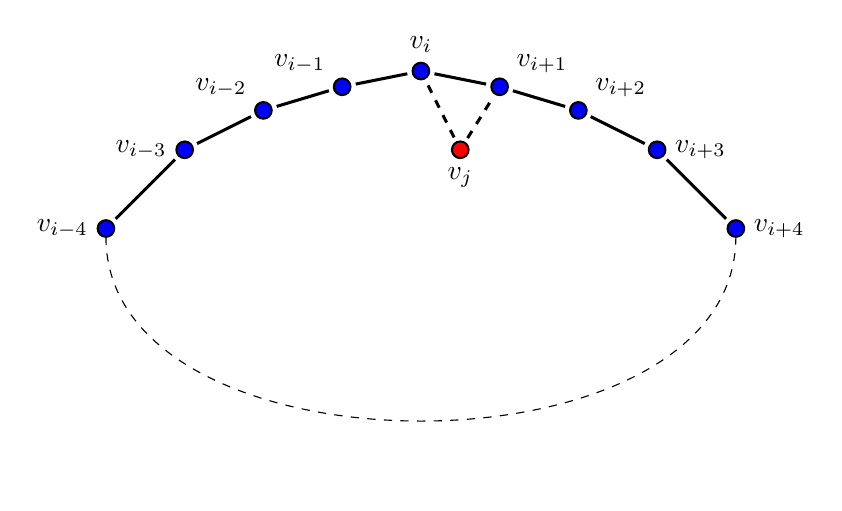
\begin{tikzpicture}
      \node(0) [blueV, label=180:$v_{i-4}$] at (-4, 3){};
      \node(1) [blueV, label=180:$v_{i-3}$] at (-3, 4){};
      \node(2) [blueV, label=150:$v_{i-2}$] at (-2, 4.5){};
      \node(3) [blueV, label=150:$v_{i-1}$] at (-1, 4.8){};
      \node(4) [blueV, label=90:$v_i$] at (0, 5){};
      \node(5) [blueV, label=0:$v_{i+4}$] at (4, 3){};
      \node(6) [blueV, label=0:$v_{i+3}$] at (3, 4){};
      \node(7) [blueV, label=30:$v_{i+2}$] at (2, 4.5){};
      \node(8) [blueV, label=30:$v_{i+1}$] at (1, 4.8){};
      \node(ext) [redV, label=270:$v_{j}$] at (0.5, 4){};
      \draw[edgeC] (0) to (5);
      \draw[edge] (0) to (1);
      \draw[edge] (1) to (2);
      \draw[edge] (2) to (3);
      \draw[edge] (3) to (4);
      \draw[edge] (4) to (8);
      \draw[edge] (5) to (6);
      \draw[edge] (6) to (7);
      \draw[edge] (7) to (8);
      \draw[edgeDotted] (ext) to (4);
      \draw[edgeDotted] (ext) to (8);
    \end{tikzpicture}
  \end{figure}
  %%%%%%%%%%%%%%%%%%%%%%%%%%%%%%%%%%%%%%%%%%%%%%%%%%%%%%%%%%%%%%%%%%%%%%%%%%
  
  \hspace*{0.5cm} \textit{Caso 2.} Existe un punto, extra en $C(S)'$ y que no esta en $C(S)$, sobre un segmento
  de $C(S)$, esto no reduce el perímetro y por tanto podemos descartar este caso.
  %%%%%%%%%%%%%%%%%%%%%%%%%%%%%%%%%%%%%%%%%%%%%%%%%%%%%%%%%%%%%%%%%%%%%%%%%% FIGURE 2
  \begin{figure}[ht!]
    \centering
    \begin{tikzpicture}
      \node(0) [blueV, label=180:$v_{i-4}$] at (-4, 3){};
      \node(1) [blueV, label=180:$v_{i-3}$] at (-3, 4){};
      \node(2) [blueV, label=150:$v_{i-2}$] at (-2, 4.5){};
      \node(3) [blueV, label=150:$v_{i-1}$] at (-1, 4.8){};
      \node(4) [blueV, label=90:$v_i$] at (0, 5){};
      \node(5) [blueV, label=0:$v_{i+4}$] at (4, 3){};
      \node(6) [blueV, label=0:$v_{i+3}$] at (3, 4){};
      \node(7) [blueV, label=30:$v_{i+2}$] at (2, 4.5){};
      \node(8) [blueV, label=30:$v_{i+1}$] at (1, 4.8){};
      \node(ext) [redV, label=270:$v_{j}$] at (0.5, 4.95){};
      \draw[edgeC] (0) to (5);
      \draw[edge] (0) to (1);
      \draw[edge] (1) to (2);
      \draw[edge] (2) to (3);
      \draw[edge] (3) to (4);
      %\draw[edge] (4) to (8);
      \draw[edge] (4) to (ext);
      \draw[edge] (ext) to (8);
      \draw[edge] (5) to (6);
      \draw[edge] (6) to (7);
      \draw[edge] (7) to (8);
    \end{tikzpicture}
  \end{figure}
  %%%%%%%%%%%%%%%%%%%%%%%%%%%%%%%%%%%%%%%%%%%%%%%%%%%%%%%%%%%%%%%%%%%%%%%%%%

  \hspace*{0.5cm} \textit{Caso 3.} Este caso lo anexo solo para estar completo,
  pero no debe suceder por la definición de $C(S)$, pues es el polígono convexo formado
  por la envolvente convexa del conjunto de puntos en $S$, así no debe haber un punto
  que no quede interno de $C(S)$ y en consecuencia de $C(S)'$.
  %%%%%%%%%%%%%%%%%%%%%%%%%%%%%%%%%%%%%%%%%%%%%%%%%%%%%%%%%%%%%%%%%%%%%%%%%% FIGURE 2
  \begin{figure}[ht!]
    \centering
    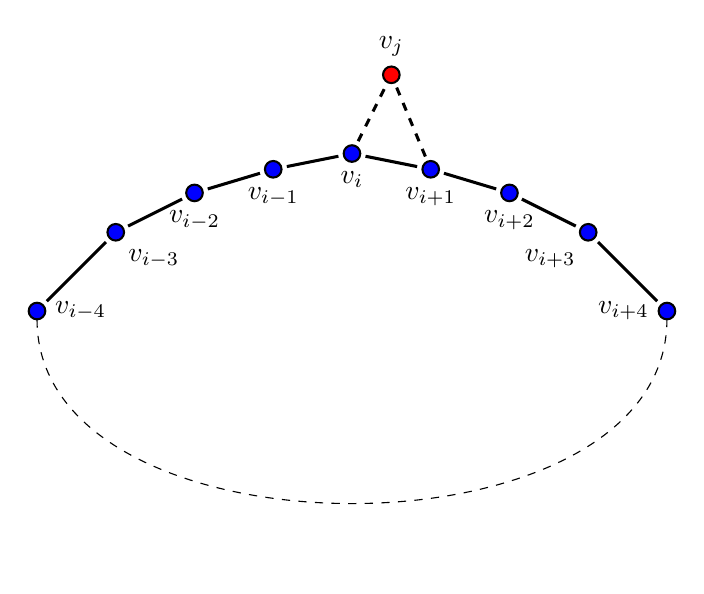
\begin{tikzpicture}
      \node(0) [blueV, label=0:$v_{i-4}$] at (-4, 3){};
      \node(1) [blueV, label=290:$v_{i-3}$] at (-3, 4){};
      \node(2) [blueV, label=270:$v_{i-2}$] at (-2, 4.5){};
      \node(3) [blueV, label=270:$v_{i-1}$] at (-1, 4.8){};
      \node(4) [blueV, label=270:$v_i$] at (0, 5){};
      \node(5) [blueV, label=180:$v_{i+4}$] at (4, 3){};
      \node(6) [blueV, label=250:$v_{i+3}$] at (3, 4){};
      \node(7) [blueV, label=270:$v_{i+2}$] at (2, 4.5){};
      \node(8) [blueV, label=270:$v_{i+1}$] at (1, 4.8){};
      \node(ext) [redV, label=90:$v_{j}$] at (0.5, 6){};
      \draw[edgeC] (0) to (5);
      \draw[edge] (0) to (1);
      \draw[edge] (1) to (2);
      \draw[edge] (2) to (3);
      \draw[edge] (3) to (4);
      \draw[edge] (4) to (8);
      \draw[edgeDotted] (4) to (ext);
      \draw[edgeDotted] (ext) to (8);
      \draw[edge] (5) to (6);
      \draw[edge] (6) to (7);
      \draw[edge] (7) to (8);
    \end{tikzpicture}
  \end{figure}
  %%%%%%%%%%%%%%%%%%%%%%%%%%%%%%%%%%%%%%%%%%%%%%%%%%%%%%%%%%%%%%%%%%%%%%%%%%

  Por lo anterior, hemos llegado a una contradicción en cada caso exhibido. Pues
  ninguno cumple ser un polígono resultado de la envolvente convexa de menor perímetro
  que $C(S)$.

  \[\therefore \text{ C(S) es de menor perímetro entre los que contienen a $S$.}\]
\item Con $C(S)$ el cierre convexo. $C(S)$ es el polígono convexo con área más pequeña, tal que
  $C(S)$ contiene a $S$.
  \newline
  Prueba por \textit{reducción al absurdo}. Analicemos los casos 1 y 2, anteriores y supongamos que
  existe $A(C(S)') < A(C(S))$.
  \begin{itemize}
  \item \textit{Caso 1}. Perdemos convexidad y por tanto llegamos a una contradicción, pues cualquier
    punto interno nos trae como consecuencia la pérdida de convexidad.
  \item \taxtit{Caso 2}. El tener un punto en un segmento no disminuye el área del polígono, por tanto
    contradice que $A(C(S)') < A(C(S))$.
  \end{itemize}
  Por lo anterior, hemos llegado a una contradicción en cada caso exhibido. Pues
  ninguno cumple ser un polígono resultado de la envolvente convexa de menor área
  que $C(S)$.

  \[\therefore \text{ C(S) es de menor área entre los que contienen a $S$.}\]
\end{itemize}

\textbf{2.} Se define el diámetro de un conjunto de puntos $S$ como la distancia más grande
entre cualesquiera dos puntos de $S$, denotado por $d$. Demuestra que d está formado por dos
vértices del cierre convexo de $S$. \newline

\textbf{\textit{Dem.}} Procedamos por inducción en el tamaño de $S$. \newline

Veamos que pasa cuándo $|S| = 3$.
\begin{figure}[ht!]
  \centering
  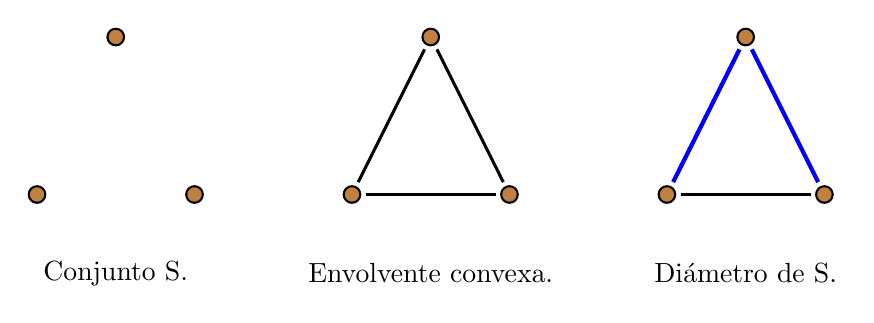
\begin{tikzpicture}
    %%%%%  Conjunto de puntos  %%%%%
    \node (0) [brownV]  at (1,1){};
    \node (1) [brownV]  at (0,-1){};
    \node (2) [brownV]  at (2,-1){};
    \node (T1)  at (1,-2) {Conjunto S.};

    %%%%% Envolvente convexa  %%%%%
    \begin{scope}[xshift=4cm]
      \node (3) [brownV]  at (1,1){};
      \node (4) [brownV]  at (0,-1){};
      \node (5) [brownV]  at (2,-1){};

      \draw [edge] (3) to (5);
      \draw [edge] (3) to (4);
      \draw [edge] (4) to (5);
      \node (T2)  at (1,-2) {Envolvente convexa.};
    \end{scope}

    %%%%% Componente debajo  %%%%%%
    \begin{scope}[xshift=8cm]
      \node (6) [brownV]  at (1,1){};
      \node (7) [brownV]  at (0,-1){};
      \node (8) [brownV]  at (2,-1){};

      \draw [blueE]  (6) to (7);
      \draw [blueE]  (6) to (8);
      \draw [edge]   (7) to (8);
      \node (T3)  at (1,-2) {Diámetro de S.};
    \end{scope}
  \end{tikzpicture}
\end{figure}
Como podemos notar, el diámetro contiene $3 > 2$ puntos.
\newline

Supongamos que cuando $|S| = k$, el diámetro de $S$ contiene dos puntos del polígono formado
por el cierre convexo de $S$.
\newline

¿Qué pasa cuándo nuestro conjunto de puntos $S$ aumenta en exactamente un punto? Existen 2 casos
interesantes para dar respuesta a esta pregunta, analicemos estos por separado
\begin{itemize}
\item Si el punto esta contenido\footnote{Casos: el punto esta al interior de $C(S)$, el punto esta en un segmento de $C(S)$.} en $C(S)$,
  terminamos. Pues, por hipótesis, nuestro diámetro ya contiene dos puntos en $C(S)$ y la anexión del punto distinguido [digamos $v$] modificaría
  al diámetro solo para aumentar $v$ (* esto lo podríamos  realizar tomando los puntos $x$ y $y$ más cercanos a $v$ que sean parte del diámetro, borar
  $xy$ de diámetro y añadir $xv$ y $vy$ a este).
  
\item Si el punto esta al exterior de $C(S)$, debemos calcular la envolvente convexa de $C(S')$, donde $S' = S + v$, esto lo podemos realizar
  econtrando las tangentes a $v$ con respecto de $C(S)$ y unirlas, este sería el nuevo cierre convexo. Lo anterior implica que $v$ será parte
  del polígono formado por la envolvente convexa (de otro modo, $v$ sería punto interno y se cubre en el caso anterior). Por ($*$) podemos anexar
  $v$ en $d$, y si el punto más cercano a $v$ es un extremo entonces basta con anexar ese segmento a $d$. Supongamos que cuando realizamos la
  unión de $v$ con $C(S)$ perdimos los puntos en $C(S)$ que también estaban en $d$ garantizados por la hipótesis, entonces ya tenemos a $v$ y como
  nadie en la envolvente pertenece a $d$, podemos anexar al vecino de $v$ en $C(S')$ a $d$ y terminamos.
\end{itemize}

\newpage

\textbf{3.} Dado un conjunto de puntos $S$ diseña un algoritmo que encuentre un polígono simple
cuyos vértices sean el conjunto $S$. \newline

\textbf{\textit{Solución.}} Para el diseño de este algoritmo tomaremos como base el algoritmo \code{Graham}
visto en clase, así, exhibamos el algoritmo
\begin{enumerate}
\item Primero debemos encontrar un punto distinguido $p_0$. Este punto puede ser cualquier punto y aquí nos podemos preguntar
  ¿Por qué cualquier punto? La respuesta es simple, todos los puntos serán parte de nuestro polígono y por tanto no da exactamente
  igual con cuál iniciar. Este paso tiene una complejidad contenida en $\mathcal{O}(1)$.
\item Ahora obtengamos un orden angular respecto a $p_0$, esto nos toma $\mathcal{O}(n \log_{2} n)$ por la cota de ordenamiento
  por comparaciones existente.
\item Ahora que ya tenemos un orden angular y un punto por el cuál iniciar, recorramos nuestros puntos tomando como siguiente, siempre,
  al próximo en el orden (así creamos una arista en cada iteración en el recorrido y lo guardamos, digamos en una lista) en sentido
  contrario a las manecillas del reloj\footnote{¿Esto necesario? No, es necesario ir en algún orden. No necesariamente este, sin embargo
  este orden es suficiente.}. Esto nos simplifica el detalle de conocer nuestras direcciones (validar) para poder regresar en caso de un
  giro en sentido contrario al requerido en \code{Graham}. Esto nos toma la cantidad de puntos en $S$, por tanto tenemos un orden
  $\mathcal{O}(n)$. Eventualmente llegaremos a $p_0$ y es en este momento que nuestro algoritmo termina regresando las aristas encontradas
  durante el recorrido.
\end{enumerate}

¿Por qué será cierto que nuestro algoritmo no encuentra aristas que se intersecten? Por el orden encontrado en ($2$).
\newline

\textit{Análisis de complejidad.} nuestro algoritmo tiene una complejidad en
\[\therefore \mathcal{O}(1) + \mathcal{O}(n \log_{2} n) + \mathcal{O}(n) \in \mathcal{O}(n \log_2 n).\]


\newpage

%%%%%%%%%%%%%%%%%%%% Problema02:
\textbf{4.} Un árbol de rango en un conjunto de $n$ puntos en el plano requiere
$\mathcal{O}(n \log n)$ de almacenamiento. Uno podría reducir los requisitos de
almacenamiento almacenando estructuras asociadas solo con un subconjunto de los
nodos en el árbol principal.

\begin{itemize}
\item Supongamos que sólo los nodos con profundidad $0, 2, 4, 6, \dotsm$ tienen
  una estructura asociada. Muestre cómo se puede adaptar el algoritmo de consulta
  para responder consultas correctamente.
\item Analice los requisitos de almacenamiento y el tiempo de consulta de dicha
  estructura de datos.
\end{itemize}

$\rhd$ \textbf{Solución:} Para este problema dividamos la solución en dos posibles
opciones:
\begin{enumerate}
\item ¿Cómo adaptamos nuestro árbol de rangos para que cumpla lo requerido en el primer
  punto? Como sabemos que un árbol, al menos, tendrá una raíz y las estructuras estarán
  ``colgadas'' de niveles pares. Entonces, la información respecto de $Y$ de los niveles
  impares estarán contenidas en el árbol colgado en su nivel par, inmediato, anterior.
  \newline
  
  Así, las consultas para los niveles pares se quedan exactamente iguales. Para los niveles
  impares consultamos respecto de $X$ y hacemos ``bracktraking'' al nivel par, inmediato,
  anterior para terminar la consulta en la estructura colgada en el nodo de ese nivel.
\item \textit{Análisis de almacenamiento.} El almacenamiento, aunque a primera vista se reduce
  en la cantidad de niveles pares, realmente las estructuras que estaban colgadas en estos niveles
  ahora formarán parte de las estructuras en niveles pares. El ahorro de almacenamiento es $\mathcal{O}(1)$,
  pues solo nos ahorramos las raíces de los niveles impares (que son, normalmente, hojas de los niveles
  pares).\newline
  
  \textit{Análisis de tiempo de consulta.} El tiempo de consulta para un elemento en un nivel par es el mismo,
  para un elemento en un nivel impar es el mismo en términos globales, pues el ``backtraking'' lo realizamos
  en tiempo $\mathcal{O}(1)$ y la consulta en la estructura ``colgada'' sigue siendo $\mathcal{O}(\log n) + k$.
  Como la consulta en árbol respecto a $X$ (árbol grande) es $\mathcal{O}(\log n)$, concluimos una
  complejidad de consulta en $\mathcal{O}(\log^2 n)$
\end{enumerate}
\textbf{Obs.} Para este problema estoy trabajando con un árbol de rango rectangulares.
\hfill $\lhd$

%\newpage
%%%%%%%%%%%%%%%%%%%%% Problema05:
\textbf{5.} Se pueden utilizar las estructuras de búsqueda de rangos ortogonales para determinar
si un punto particular $(a, b)$ está en un conjunto dado, haciendo una consulta al rango
$[a : a] \times [b : b]$.
\begin{enumerate}
\item[$a$)] Prueba qué hacer una consulta así en un árbol $Kd$ toma tiempo $\mathcal{O}(\log n)$.
\item[$b$)] ¿Cuál es la complejidad para una consulta así en un árbol de rangos?
\end{enumerate}

$\rhd$ \textbf{Solución:} Para este problema dividamos la solución en dos posibles casos:
\begin{enumerate}
\item[$a$)] Sabemos que hacer una consulta, en un árbol $Kd$, para un rango en
general nos toma $\mathcal{O}(\sqrt{n} + k)$. Sin embargo, consultar un punto
en un árbol $Kd$ sería equivalente a particionar la nuve de puntos por la mitad
y preguntarnos en qué parte queda nuestro punto distinguido, llamemosle $q$. Así,
descartamos aproximadamente la mitad de puntos en dónde no se encuentra $q$. Luego,
subdividimos nuevamente el conjunto de puntos restantes en $2$ y nos preguntamos
en qué parte se encuentra $q$ y podemos descartar la parte en la que no se encuentre.
De esta manera y recursivamente nuestro espacio de búsqueda se reduce a la mitad cada
vez, esto equivale hacer un recorrido de la raíz de nuestro árbol $kd$ hacia las hojas
en búsca del punto $q$. Como cada vez descontamos la mitad del conjunto de puntos
de búsqueda, tenemos la recurrencia $T(n) = 2T(n - 1)$ que sabemos que nos genera
un orden logarítmico en base 2. Cómo el número de consultas es igual a $1$, entonces
$k = 1 \in \mathcal{O}(1)$. Por tanto, la complejidad de esta consulta es
$\mathcal{O}(\log n)$.
\item[$b$)] En este caso, tenemos una complejidad general de $\mathcal{O}(\log^2 n + k)$,
cómo solo estamos consultando un punto y no un rango, entonces $k = 1 \in \mathcal{O}(1)$.
En la consulta debemos bajar por el árbol hasta encontrar $q.X$ y bajar su árbol ``colgado''
o su árbol asociado en $y$, hacer esto es igual a $\log m$ dónde $m$ es la altura del árbol
asociado con $m \not= n$, pues cada nivel y nodo tiene un árbol compacto de tamaño constante.
Por tanto, la complejidad esta contenida en $\mathcal{O}(\log m \cdot \log n) = \mathcal{O}(\log n)$
con $m$ constante respecto de $n$.

\end{enumerate}
\hfill $\lhd$

%\textbf{Dem. ($a$):} 
Procedemos por inducción.

Observemos que cuando tenemos un solo círculo se cumple por vacuidad. Con $2$ círculos,
  %%%%%%%%%%%%%%%%%%%%%%%%%%%%%%%%%%%%%%%%%%%%%%%%%%%%%%%%%%%%%%%%%%%%%%%%%% FIGURE 1
  \begin{figure}[ht!]
    \centering
    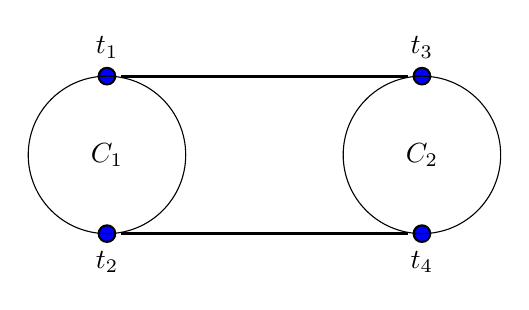
\begin{tikzpicture}
        %\draw [line width=1pt, dash pattern=on 1pt off 2pt] (9,6) circle(1);
        \node(0) at (2, 2){$C_1$}; %[blueV, label=180:$t_1$]
        \node(1) at (6, 2){$C_2$}; %[blueV, label=180:$t_1$]
        \node(t1) [blueV, label=90:$t_1$] at (2, 3){};
        \node(t3) [blueV, label=90:$t_3$] at (6, 3){};
        \node(t2) [blueV, label=270:$t_2$] at (2, 1){};
        \node(t4) [blueV, label=270:$t_4$] at (6, 1){};
        \draw (0) circle (1cm);
        \draw (1) circle (1cm);
        \draw[edge] (t1) to (t3);
        \draw[edge] (t2) to (t4);
     \end{tikzpicture}
  \end{figure}
  %%%%%%%%%%%%%%%%%%%%%%%%%%%%%%%%%%%%%%%%%%%%%%%%%%%%%%%%%%%%%%%%%%%%%%%%%%

$C_1$ y $C_2$, obtenemos
tangentes a cada circunferencia, por cada circuferencia en $2$ puntos distintos. A partir de los puntos de
tangencia con $C_1$ y hasta la frontera externa tenemos un ''pedacito'' de circulo (caso análogo con $C_2$ y
$t_2$, $t_4$). Las tangentes $t_1t_3$ y $t_2t_4$ son las rectas y por tanto terminamos. \newline

\textbf{H.I.} Supongamos que el cierre convexo esta formado por ``pedacitos'' de círculo y rectas, para $k$ círculos. \newline

¿Qué pasa si introducimos un círculo más? Los posibles casos son:
\begin{enumerate}
    %%%%%%%%%%%     1
    \item El nuevo círculo queda contenido en el cierre convexo. En este caso y por H.I tenemos que
    el cierre convexo \textbf{No} se ve modificado y terminamos.
    %%%%%%%%%%%     2
    \item El nuevo círculo queda como frontera. Por H.I, el cierre ya se forma por ''pedacitos''
    de círculos y segmentos de rectas, además el nuevo círculo anexa
    \begin{itemize}
        \item una parte de su contorno y dos segmentos tangentes del anterior cierre al nuevo círculo y por tanto terminamos.
        \item O es parte de la frontera en un solo punto y por \textbf{H.I.} terminamos. \hfill$\square$
    \end{itemize}
\end{enumerate}

%\textbf{Dem. ($b$):} Procedamos por reducción al absurdo.

Supongamos que un círculo puede estar al menos $2$ veces en el contorno del cierre convexo.
Entonces, existe un círculo $C$ que tiene al menos \textbf{2 arcos} sobre el contorno del
cierre convexo. Si esto fuese cierto, tendríamos que hay más de $2$ tangentes sobre $C$ tal
que \textbf{No} se intersectan, como cada tangente a $C$ debe ser parte del contorno,
%%%%%%%%    Dibujo    %%%%%%%%%
 entonces puede pasar que:
%%%%%%%%    Dibujo    %%%%%%%%%
\begin{enumerate}
    %%%%%%%%%%%%    1   %%%%%%%
\item Hay un círculo que \textbf{No} pertenece al cierre, pues es dejado fuera por una tangente (digamos
  que las dos más juntas hacen el cierre). Hasta aquí hemos llegado a una contradicción por suponer que
  hay un círculo con al menos dos arcos en el cierre convexo.
    %%%%%%%%%%%%    2   %%%%%%%%
\item Los círculos son parte del cierre, y por tanto perdemos convexidad. Nuevamente hemos llegado
  a contradecir lo supuesto.
\end{enumerate}

¿Por qué perdemos convexidad?\\
%%%%%%%%    Dibujo    %%%%%%%%%
Como hemos dicho, nuestro círculo esta al menos $2$ veces en el contorno, esto implica que
hay al menos $3$ tangentes al círculo que son parte del contorno y que \textbf{No} son
contiguas (si lo fuera serían una sola recta en vez de $2$). Como $2$ segmentos \textbf{No}
son contiguos, entonces, NO existe el caso donde hayan dos rectas contiguas tales que formen
un ángulo de $180°$
%%%%%%%%    Dibujo      %%%%%%%%
y por tanto una recta (o segmento prolongado) \textbf{siempre} puede cortar los $3$ segmentos
tangentes a $C!$, pues si esto NO sucediera, implicaría que una de las (segmentos) rectas
esta contenida por otras $2$ y esto es falso, pues supusimos que las $3$ son parte del contorno.\\
%%%%%%%%    Dibujo      %%%%%%%%
\[
\therefore \text{ Un círculo esta a lo más una vez en el contorno de cierre convexo.}
\]

%\textbf{Dem. ($c$):} Análicemos dos posibles casos:
\begin{itemize}
\item[$\Rightarrow )$] Procedemos por reducción al absurdo.
  
 Nota: $C(S)$ el cierre de $S$ y $C(S')$ el cierre de $S'$
 Supongamos que en $C(S)$ se encuentra $C_i$ como parte de su contorno y $O_i$ 
 (centro de $C_i$). No esta $C(S')$, esto implica que:

 \begin{enumerate}
     \item $O_i$ queda fuera de $C(S')$, esto \textbf{No} se admite, pues $C(S')$
     es el cierre convexo.
     \item $O_i$ \textbf{No} es parte del contorno de $C(S')$ y queda interno, por tanto
     existe $O_j$ que es más ''externo'' que $O_i$, esto implica que $C_j$ es más externo
     que $C_i$ (recordando que los círculos son unitarios) pero $C_i$, es parte del contorno.
     
     He aquí una contradicción de suponer que $O_i\notin C(S')$.
 \end{enumerate}

\item[$\Leftarrow )$] Procedamos por reducción al absurdo.
  
Sea $C(S')$ el cierre convexo de $S'$ y $C(S')$ el cierre convexo de $S$. 
Si $O_i\in C(S')\Rightarrow C_i\notin C(S)$ para algún $i\in [1,...,n]$ y 
$O_i$ corresponde al centro de $C_i$.\\

Como $C_i$ \textbf{No} es parte de $C(S)$, entonces existe $C_j$ más ''externo'' que 
$C_i$ y por tanto $O_j$ es más ''externo'' que $O_i$, pues son círculos unitarios, 
esto contradice el hecho de que $O_i\in C(S')$ refiriendonos a que forma parte de su 
contorno, pues $O_j$ queda fuera de $C(S')$ y $O_j$ es elemento de $S'$. Lo anterior contradice
el hecho de que $O_i$ era parte de la frontera de $C(S').$\\
\end{itemize}
De aquí concluimos lo que se quería mostrar. \hfill $\square$
\newline


%\textbf{Solución (d):}
Este algoritmo estará basado fuertemente en el algoritmo de Graham. A continuación
se exhibe el algoritmo requerido:
 \begin{enumerate}
     \item Aplicar Graham en el conjunto de centros de cada círculos $S'$. Esto nos
     toma $O(n \log_2 n)$
     \item Obtenemos las paralelas de $C(S')$ en exactamente una unidad, por el
     inciso  $c)$ sabemos que las círcunferencias de estos puntos forman el cierre
     convexo $C(S)$. Esto nos toma $O(n)$.
     \item Por cada recta paralela, digamos $\ell_{i} 's$ tomemos sus extremos en un
       sentido $\rightarrow$ y recorremos desde ese punto por los pedacitos de círcunferencia
       a donde son tangentes (por a,b,c) hasta encontrarse con la otra recta, así unimos ese
       pequeño arco. Esto lo hacemos en $\mathcal{O}(n)$.
 \end{enumerate}

El resultado de estos pasos es el cierre convexo de $S$.\newline

\textit{Análisis de complejidad.} La complejidad esta contenida en
\[
\mathcal{O}(n \log n) + \mathcal{O}(n) + \mathcal{O}(n) = \mathcal{O}(n \log n).
\]

%\newpage
%%%%%%%%%%%%%%%%%%%%% Problema06:
\textbf{6.} En algunas aplicaciones solo nos interesa el número de puntos que caen dentro de
un rango y no reportar cada uno de ellos. En este caso nos gustaría evitar el término
$\mathcal{O}(k)$ en el tiempo de consulta.
\begin{enumerate}
\item[$a$)] Describe cómo un árbol de rangos de una dimensión puede adaptarse para que
una consulta así se pueda realizar en tiempo $\mathcal{O}(\log n)$.
\item[$b$)] Usando la solución al problema para una dimensión, describe cómo se pueden
responder consultas de conteo en rangos de $d$ dimensiones en tiempo $\mathcal{O}(\log^d n)$.
\item[$c$)] Describe cómo se puede usar la técnica de cascada para mejorar el tiempo de
consulta en un factor $\mathcal{O}(\log n)$ para dos y más dimensiones.
\end{enumerate}

$\rhd$ \textbf{Solución:} A continuación se da solución a cada uno de los incisos:
\begin{enumerate}
\item[$a$)] La versión para una dimensión sería bastante simple, y de hecho sería
  como un árbol binario de búsqueda balanceado, pues basta con preservar el árbol
  general sin los árboles ``colgados'' que tiene el árbol de búsuqeda ortogonal.
  \newline
  
  La manera de ahorrar $\mathcal{O}(k)$ durante la búsqueda de rango, sería no recorrer las
  hojas del rango encontrado. Pues, basta con realizar dos recorridos hacia abajo desde la
  raíz, uno para encontrar la cota inferior del rango y otro para encontrar la cota superior.
  Así, y por la propiedad de tener mayores a la derecha y menores a la izquierda concluimos
  que las hojas entre las seleccionadas forman parte del rango.
\item[$b$)] De la misma manera, que en el caso de una dimensión, nos ahorramos $\mathcal{O}(k)$
  al no recorrer las hojas que quedan dentro del rango. Para generalizar a $d$ dimensiones basta
  reproducir la idea de los árboles ``colgados'', pues cada nodo que no sea hoja tendrá, inicialmente
  una referencia al árbol con coordenadas en $Y$. Luego los árboles con coordenadas en $Y$ tendrán
  colgados árboles con coordenadas en $Z$, y así de manera recursiva. Cuándo se requiera obtener
  el rango bastará con bajar por el árbol principal y recorrer cada árbol asociado de manera
  recursiva para inspeccionar que efectivamente el punto quede dentro del rango requerido.
  Cómo recorremos $\log n$ el árbol principal y por cada nodo distinto a una hoja recorremos
  su árbol asociado y a su vez los asociados recursivamente, entonces tenemos una complejidad
  de $k \cdot \log n$ dónde $k = \log m \cdot \log m' \dotsm \log m^{\dotsm} \approx \log^{d - 1} n$
  y concluimos que la complejidad en general por recorrido para encontrar un punto en el rango
  es de $\mathcal{O}(\log^d n)$.\newline
  
  Como esto se tiene que hacer para el punto ``menor'' en el rango y para el punto ``mayor''
  en el rango,  entonces tenemos una complejidad contenida en
  \[2 \cdot \mathcal{O}(\log^d n) \in \mathcal{O}(\log^d n).\]
\item[$c$)] 
\end{enumerate}
\hfill $\lhd$

%\newpage
%%%%%%%%%%%%%%%%%%%%% Problema07:
\textbf{7.} Da un algoritmo que calcule en tiempo $O(n \log n)$ una diagonal que divida un
polígono simple con $n$ vértices en dos polígonos simples cada uno con a lo más
$\lfloor \frac{2n}{3} \rfloor + 2$ vártices. \textbf{Hint}: Usa la gráfica dual de la triangulación.
\newline

$\rhd$ \textbf{Solución:} A continuación se exhibe un algoritmos que resuelve este problema
\begin{enumerate}
\item Obntener la triangulación de nuestro polígono. Esto lo realizamos en $\mathcal{O}(n \log n)$
  con el algoritmo visto en clase.
\item Sabemos que toda triangulación tiene $n - 3$ aristas y por tanto nuestra gráfica dual que
  se formará a partir de cada arista interna será de un orden $\mathcal{O}(n)$. Entonces, la
  construcción de la gráfica dual nos toma $\mathcal{O}(n)$. Además, la gráfica dual es un árbol.
\item Encontramos los puntos más lejanos en una gráfica. Esto, por algoritmos $I$ sabemos que
  lo podemos hacer en $\mathcal{O}(n)$ para un árbol. La técnica se basa en ``colgar'' el árbol
  por medio de un recorrido a profundidad desde la raíz hasta la hoja de mayor profundidad y
  tomar esa hoja como la nueva raíz y volver a recorrer hasta la hoja más profunda.
\item  Recorrer la gráfica dual iniciando desde cada uno de los puntos más lejanos. Eligimos una
  orientación y siempre seguimos esta orientación (La orientación, la podemos tener con DCEL) para
  el reccorido. Así evitaremos dividir el polígono en más de $2$ polígonos nuevos. Esto lo hacemos
  en $\mathcal{O}(n)$, pues el orden de las aristas de nuestra gráfica dual es lineal.
\item Durante cada recorrido colorearemos los vértices del triángulo en el que estemos, todos
  del mismo color. En el momento que hayamos coloreado, exactamente $\lfloor \frac{2n}{3} \rfloor + 2$
  vértices. Entonces regresamos la arista $e_T$ de la triangulación por la que fue creada la arista
  siguiente a la última hasta haber coloreado los  $\lfloor \frac{2n}{3} \rfloor + 2$ vértices.
  Esto lo hacemos en $3 \cdot \left( \lfloor \frac{2n}{3} \rfloor + 2\right)$ pasos que obedece
  a un orden líneal.\newline
  
  ¿Con cuál recorrido nos quedamos? Con el que llegue primero a colorear los $\lfloor \frac{2n}{3} \rfloor + 2$
  vértices y cumpla que la arista divide al polígono en las características deseadas.\newline

  \textbf{Obs.} Podríamos hacer una versión con $\lfloor \frac{n}{3} \rfloor - 2$ tomandolo por cota.
\end{enumerate}
Al final, $e_T$ es la diagonal búscada.\newline

\textit{Análisis de la complejidad.} La complejidad del algoritmo esta contenida en
\[\mathcal{O}(n \log n) + \mathcal{O}(n) = \mathcal{O}(n \log n).\]
\hfill $\lhd$

%\newpage
%\textbf{8.} Suponga que se tiene una lista de aristas doblemente ligada (DCEL) de una subdivisión
plana. Diseña un algoritmo que encuentre todas las caras que contienen un vértice en la cara exterior.
\newline

\textbf{Solución.} A continuación se exhibe el algoritmo requerido:
\begin{enumerate}
\item Ordenamos la lista de aristas (DCEL), esto nos toma $\mathcal{O}(n \log n)$.
\item Encontremos el punto más ``chico'' en nuestro polígono. Esto lo realizamos en $\mathcal{O}(1)$,
  pues hemos ordenado nuestras aristas.
\item Recorramos siempre hacia la izquierda excepto cuando:
  \begin{enumerate}
  \item El vértice al que llegamos no pertenece a una cara externa. En este caso nos regresamos
    y ahora tomamos el camino más a la derecha.
  \item El vértice de llegada es el vértice de partida, entonces hemos llegado y terminamos.
  \end{enumerate}
  Durante el recorrido vamos acumulando los vértices que sean externos en una lista, como el recorrido
  esta dado por las aristas DCEL esto nos toma a lo más tiempo $\mathcal{O}(n)$. Pues cuando lleguemos a un vértice
  interno de inmediato nos regresamos.
  
  ¿Cómo sabemos que el vértice pertenece o no a la cara externa? La arista nos lo indica.
\end{enumerate}

\textit{Análisis de complejidad}. La complejidad de este algoritmo esta contenida en
\[\mathcal{O}(n \log n) + \mathcal{O}(n) + \mathcal{O}(1) = \mathcal{O}(n \log n).\]


\end{document}
